\documentclass[11pt]{article}
\usepackage{graphicx}
\usepackage{hyperref}
\usepackage{natbib}

\setlength{\textwidth}{6.5in}
\setlength{\headheight}{0in}
\setlength{\textheight}{8.0in}
\setlength{\hoffset}{0in}
\setlength{\voffset}{0in}
\setlength{\oddsidemargin}{0in}
\setlength{\evensidemargin}{0in}

\title{Computational Physics HW1 P3}
  
\author{Siyuan Chen}


\begin{document}

\maketitle

\section*{}
Computer is a crucial tool for research. From this course, I want to have a glance of its general applications in research and gain resources which I could learn things in more details when I need to use them later. I have done some simulation in matlab before and some simple projects with python. I just started my PhD program, so I'm not sure what I'll do after it. For my PhD, I'm looking for an interesting project in soft matter field.

\begin{figure}
    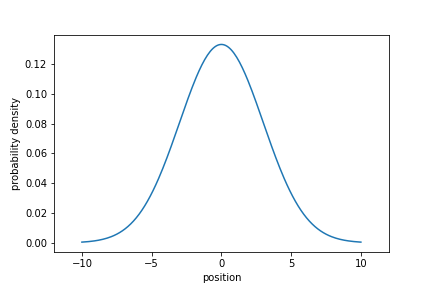
\includegraphics{gaussian.png}
    \caption{\textbf{Gaussian Distribution} This is a Gaussian plot from problem 2 of this assignment. It is of mean $\mu=0$ and standard deviation $\sigma=3$ over range $[-10,10]$.
    }
    \label{fig}
\end{figure}

\section*{}
My GitHub account: Chessy7

\end{document}

 
 
